\subsection{Results}
\label{ssec: Results}

The resulting annualized costs and CO$_2$ emissions for all investigated scenarios are shown in Fig.~\ref{fig: pareto set}.
The full black line displays the Pareto set and the cross stands for the traditional BES design.
Circles mark the CHP scenarios, diamonds the PV scenarios, stars the forced installation of a HP and rectangles the BAT scenarios.
Red markers represent scenarios in which subsidies are considered and blue markers show the results for not using the available subsidies.
The following subsections describe the results of each scenario in more detail.

\begin{figure}[h!]
	\begin{center}
		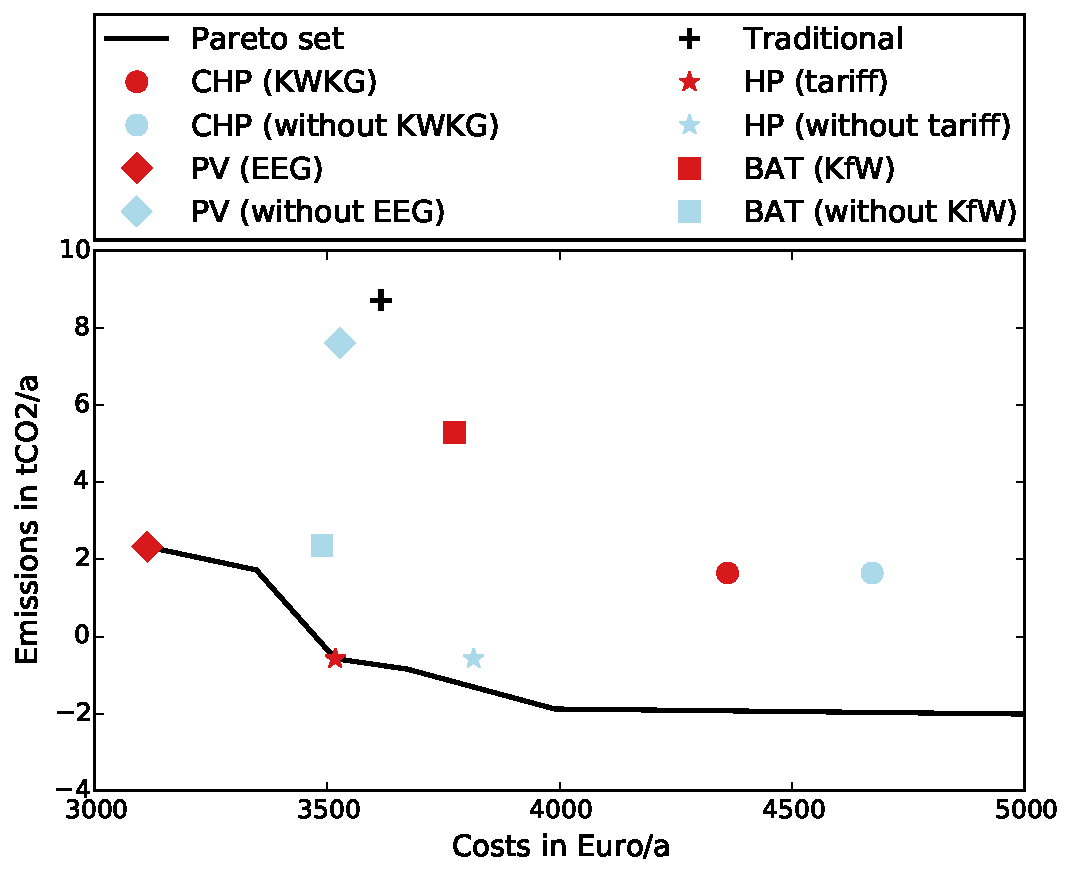
\includegraphics[width=\linewidth]{figures/pareto_set.pdf}
		\caption{Annualized costs and emissions (single column figure)}
		\label{fig: pareto set}
	\end{center}
\end{figure}

\subsubsection{Pareto set}
The Pareto set describes all solutions in which the costs can only be reduced at the expense of increased CO$_2$ emissions, therefore no solution can simultaneously decrease costs and CO$_2$ emissions below this frontier.
The cost optimal solution, which also coincides with the PV with EEG scenario (red diamond), requires 3140~EUR and causes 2.38~tons of CO$_2$ per year.
On the other hand, the optimal solution regarding emissions, costs 8410~EUR and emits -2.68~tons of CO$_2$.
Between these two limits, we calculated five additional points to approximate the Pareto curve.

The installed rated powers of each point of the Pareto curve are displayed in Fig.~\ref{fig: heat generation moo}.
For all optimizations, a 14.2~kW boiler is chosen that functions as a primary heat generator for cost efficient solutions and as a backup unit for low emission solutions.
Additionally, small EH devices are purchased as inexpensive, electricity driven heat generators that utilize excess electricity produced from PV units.
Such PV units are installed in every point of the Pareto set.
The installed PV peak power is 11.2~kW for cost optimal solutions and increases with rising focus on emissions to 13.5~kW.
Further additions of PV are not possible due to the limited available roof area.
With increasing focus on emissions, heat is mostly generated through HP units.
Only in the minimal emissions calculation, a small CHP unit is purchased.
The only time a

\begin{figure*}[h!]
	\begin{center}
		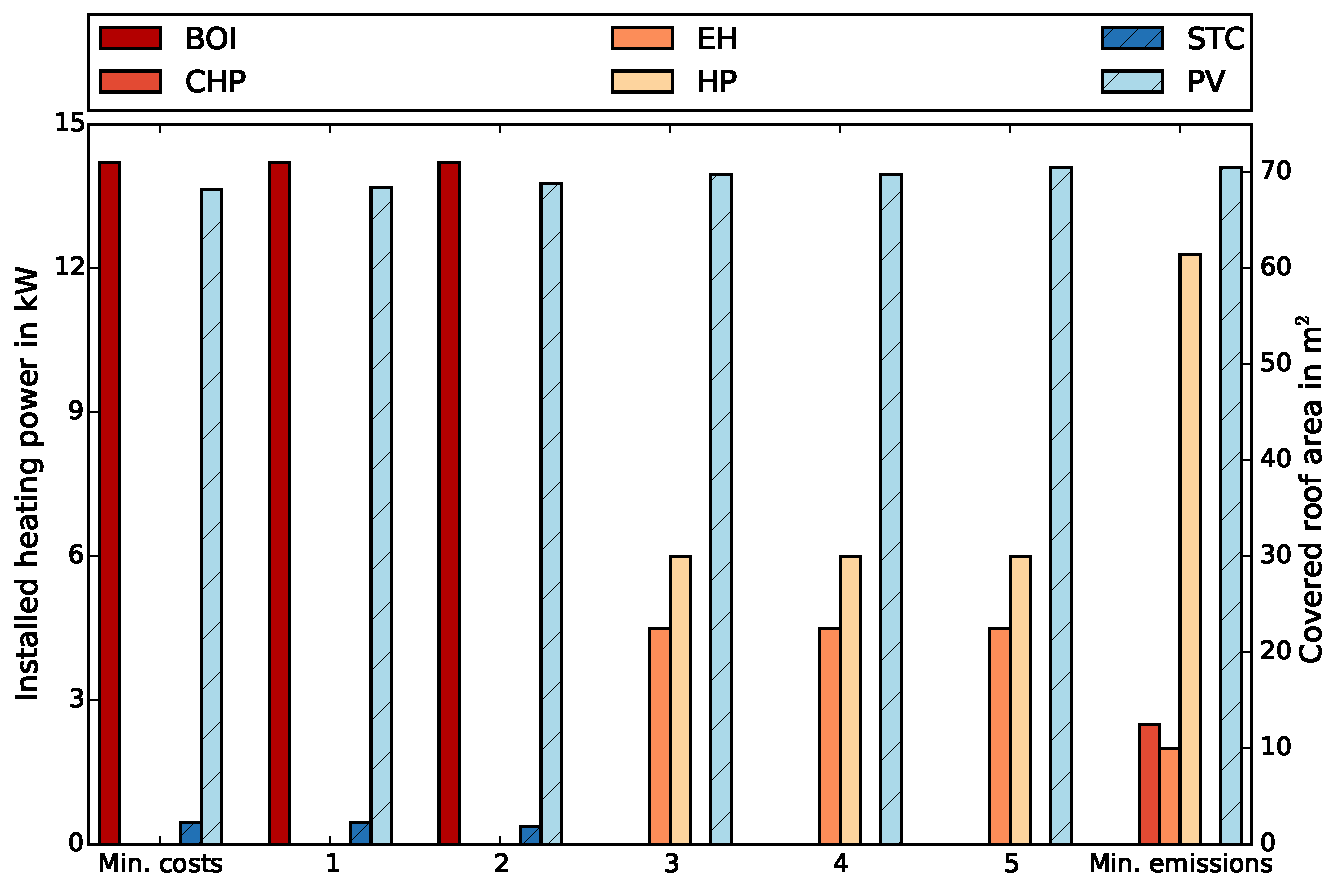
\includegraphics[width=\linewidth]{figures/plot_cap_gen_moo.pdf}
		\caption{Rated powers (Pareto set) (double column figure)}
		\label{fig: heat generation moo}
	\end{center}
\end{figure*}

Fig.~\ref{fig: cap storage moo} shows the installed capacities of storage units.
Red bars display the water volume of TES units and blue bars the capacity of BAT.
Pure cost minimization leads to the installation of a small scale TES unit, but with increasing importance of emissions, the TES volume is increased.
The jump from approx. 0.1~m$^3$ in the cost optimal solution to 0.6~m$^3$ in optimization~1 is also due to the installation of a small scale STC unit that provides 1.9\% of the annual thermal demand.
Larger TES volumes also allow for shifting the HP's operation to times with higher PV availability, reducing grid dependency.
In the minimum emissions calculation, a large BAT system is installed allowing for even more flexible operations.

\begin{figure}[h!]
	\begin{center}
		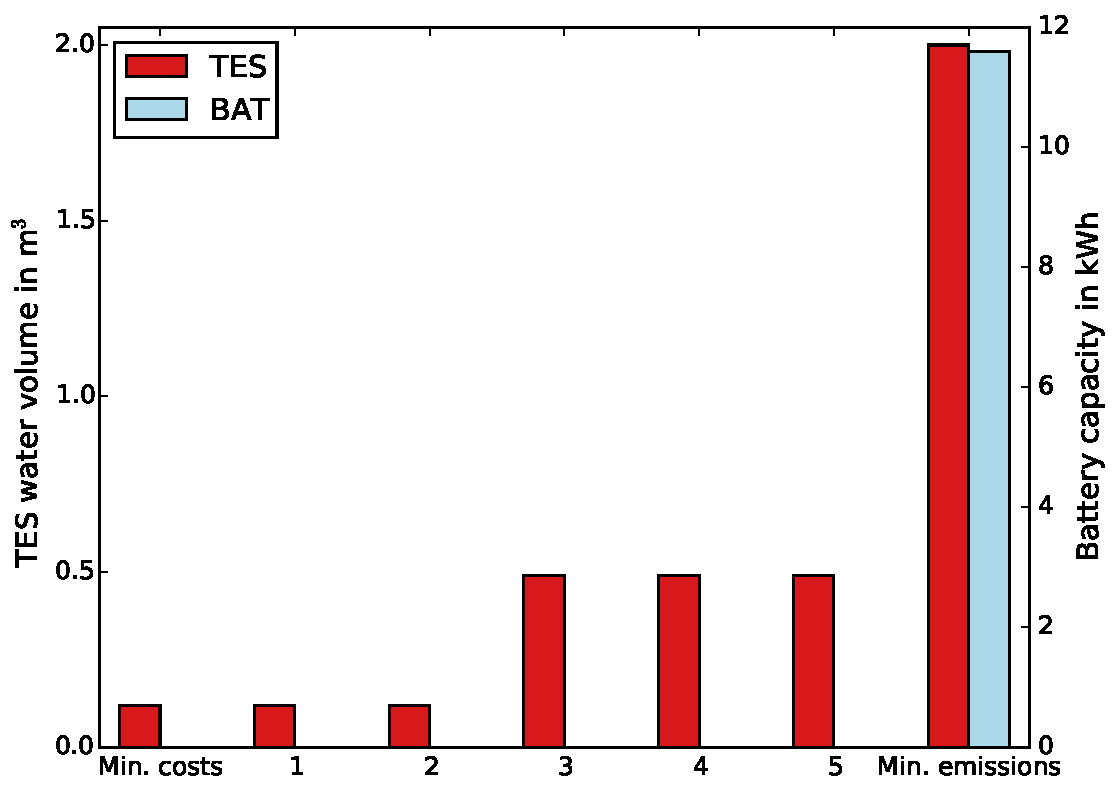
\includegraphics[width=\linewidth]{figures/plot_cap_sto_moo.pdf}
		\caption{Capacities of storage devices (Pareto set) (single column figure)}
		\label{fig: cap storage moo}
	\end{center}
\end{figure}

The heat coverage ratios for the Pareto efficient optimizations are depicted in Fig.~\ref{fig: heat coverage moo}.
In the minimum cost case, more than 99.6\% of the annual thermal demand is covered with the boiler, the rest is generated through the backup EH.
With increasing awareness of emissions, the boiler's usage is reduced.
Initially, in optimization~1, it is marginally substituted with an STC that contributes 1.9\% of the heating demand.
After installation of a HP in optimization~2, the boiler mainly serves as a backup unit that provides approx. 10\% of the heating demand.
In the minimum emissions case, a CHP unit is installed additionally.
In this case, 99.5\% of the annual thermal demand is generated with either CHP or HP.

The self-consumption rate of electricity generated locally with either CHP or PV increases from 10\% in the most cost-efficient optimization to approx. 20\% when a HP is installed. 

\begin{figure}[h!]
	\begin{center}
		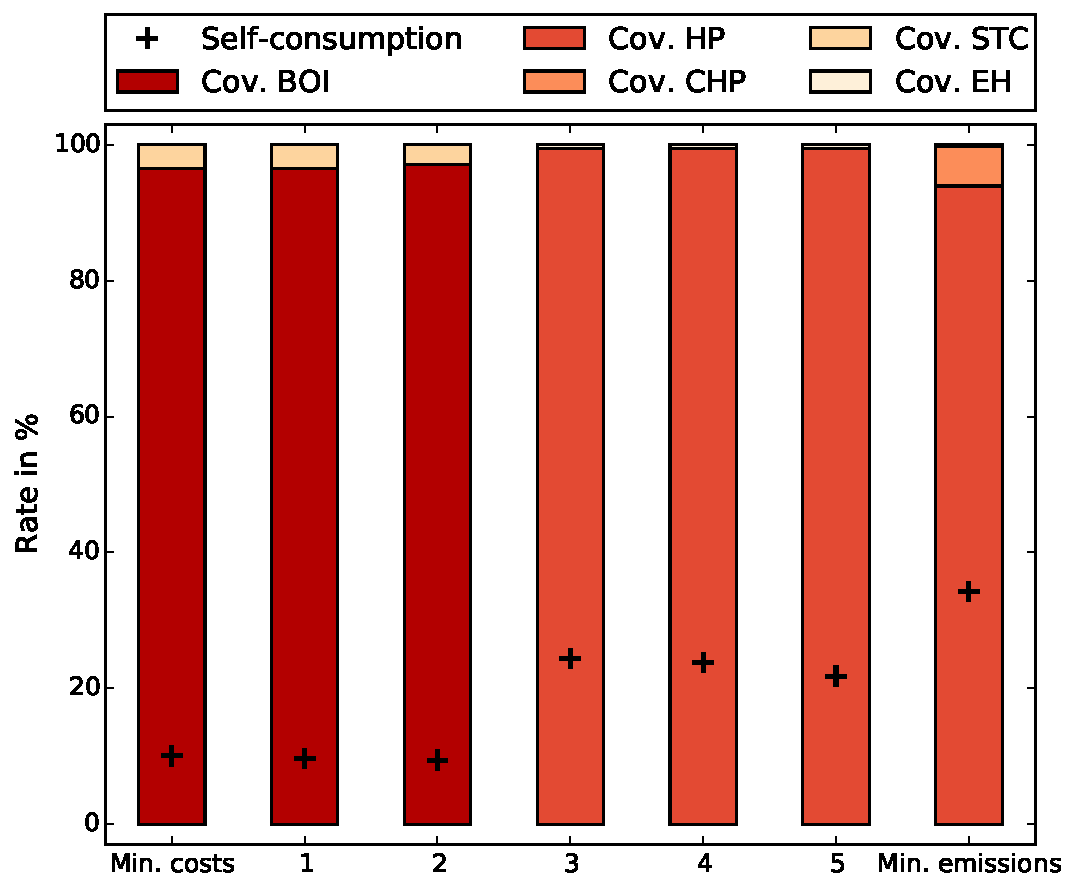
\includegraphics[width=\linewidth]{figures/plot_coverage_moo.pdf}
		\caption{Heat coverages (Pareto set) (single column figure)}
		\label{fig: heat coverage moo}
	\end{center}
\end{figure}






\subsubsection{Traditional scenario}
The black cross in Fig.~\ref{fig: pareto set} marks the result of the traditional scenario.
In comparison with the other cases, this scenario leads to the highest CO$_2$ emissions of 8.71~tons per year.
The annualized costs are 3616~EUR.
The BES consists of a 14.20~kW boiler and a TES with 0.12~m$^3$ of water volume.
Since on-site generation through PV or CHP units is prohibited, the entire electricity amount of 4000~kWh/a is bought from the distribution grid.



\subsection{PV scenarios}
In Fig.~\ref{fig: pareto set}, the diamonds represent the PV scenarios.
Red color indicates that the corresponding restrictions, in this case the subsidies according to the German Renewable Energy Sources Act, are activated, while blue markers stand for deactivated subsidies.


\subsubsection{CHP scenarios}
In Fig.~\ref{fig: pareto set}, the circles represent the CHP scenarios.
Red color indicates that the corresponding restrictions, in this case the subsidies according to the German Cogeneration Act, are activated, while blue markers stand for deactivated subsidies.
In both cases, the same BES comprising a 2.50~kW CHP unit, a 14.20~kW boiler and a 4.5~kW backup resistance heater are used to cover the thermal loads.
Furthermore, a 0.49~m$^3$ TES unit and 69.8~m$^2$ of PV area are installed.

The devices' operation is barely affected by the subsidies.
Both scenarios achieve approx. 4400 full load hours for the CHP unit and run this device electricity driven, leading to 



\begin{figure}[h!]
	\begin{center}
		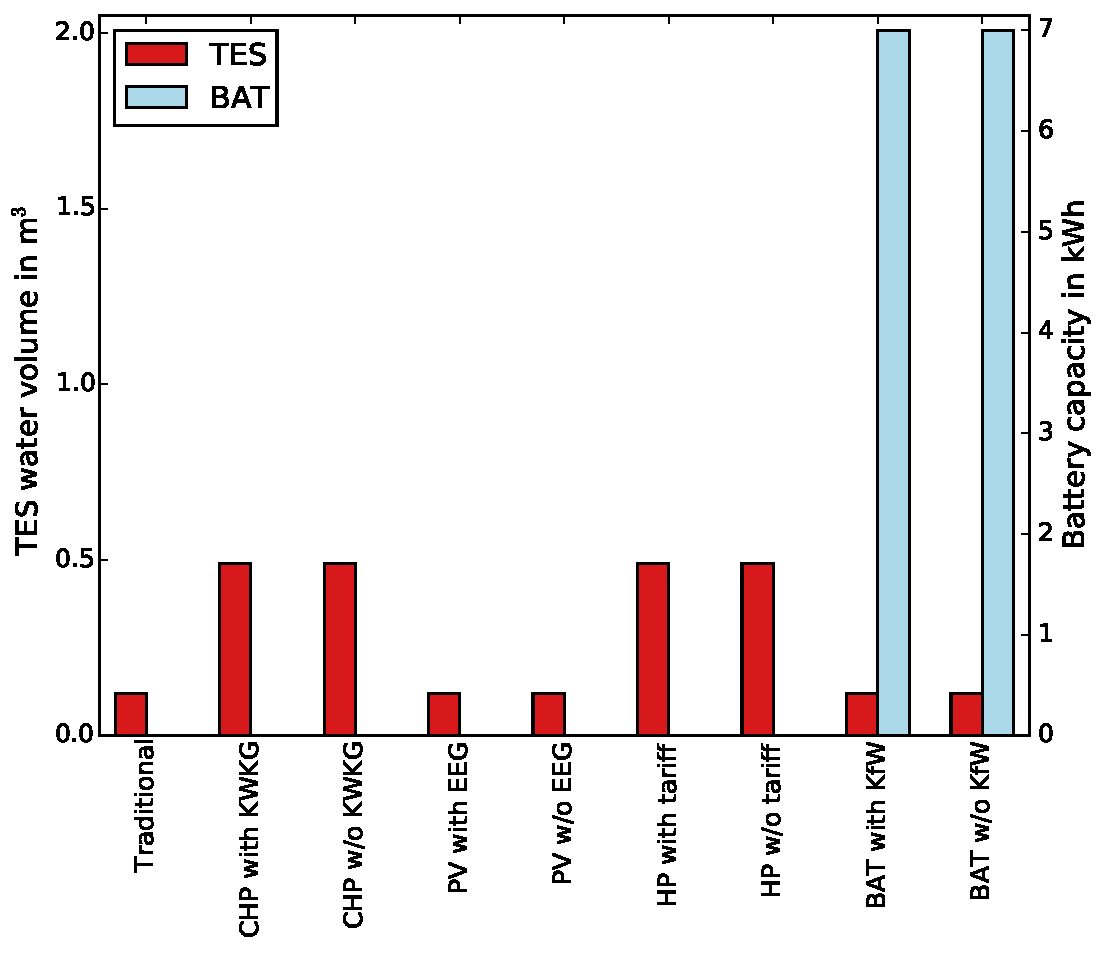
\includegraphics[width=\linewidth]{figures/plot_cap_sto_other.pdf}
		\caption{Capacities of storage devices (rest) (single column figure)}
		\label{fig: cap storage other}
	\end{center}
\end{figure}



\begin{figure}[h!]
	\begin{center}
		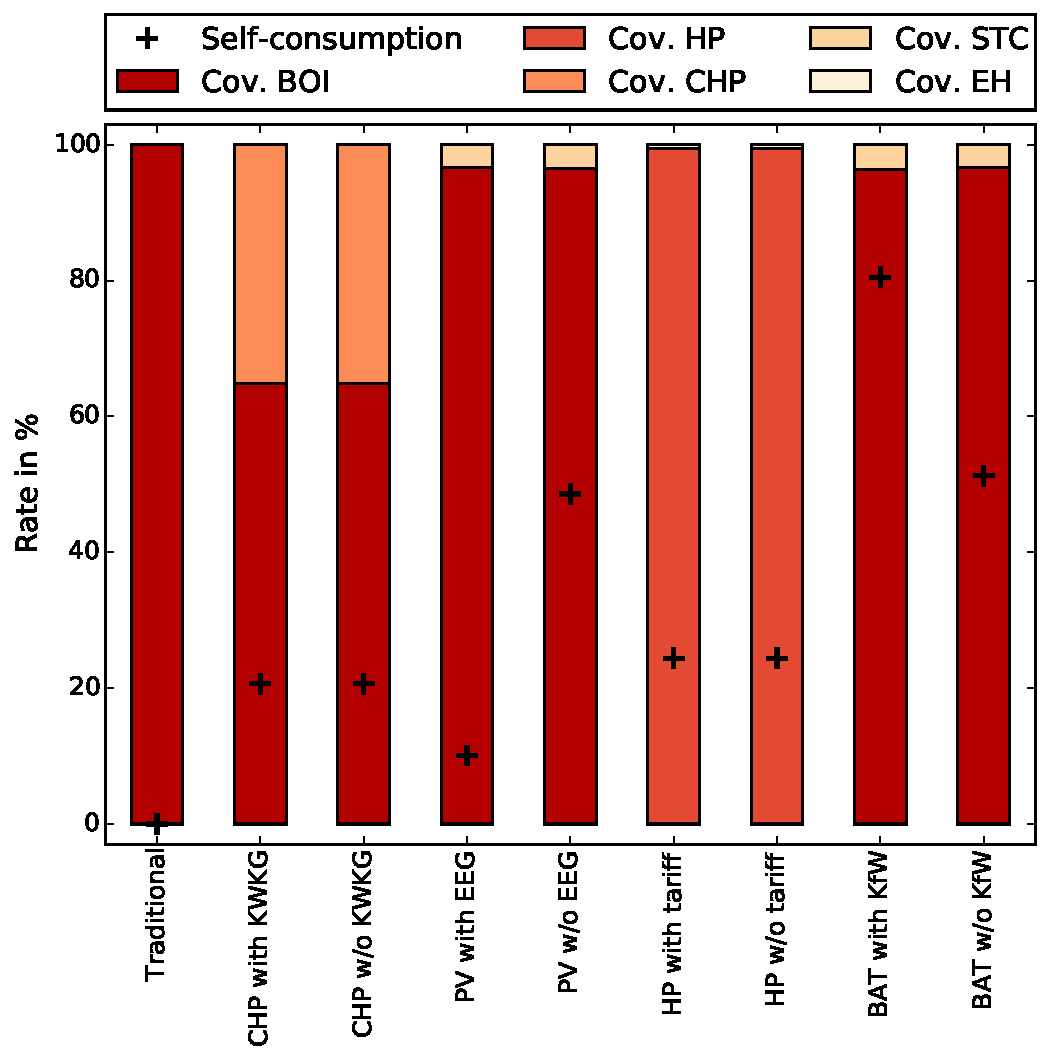
\includegraphics[width=\linewidth]{figures/plot_coverage_other.pdf}
		\caption{Heat coverages (other) (single column figure)}
		\label{fig: heat coverage other}
	\end{center}
\end{figure}



\begin{figure*}[H!]
	\begin{center}
		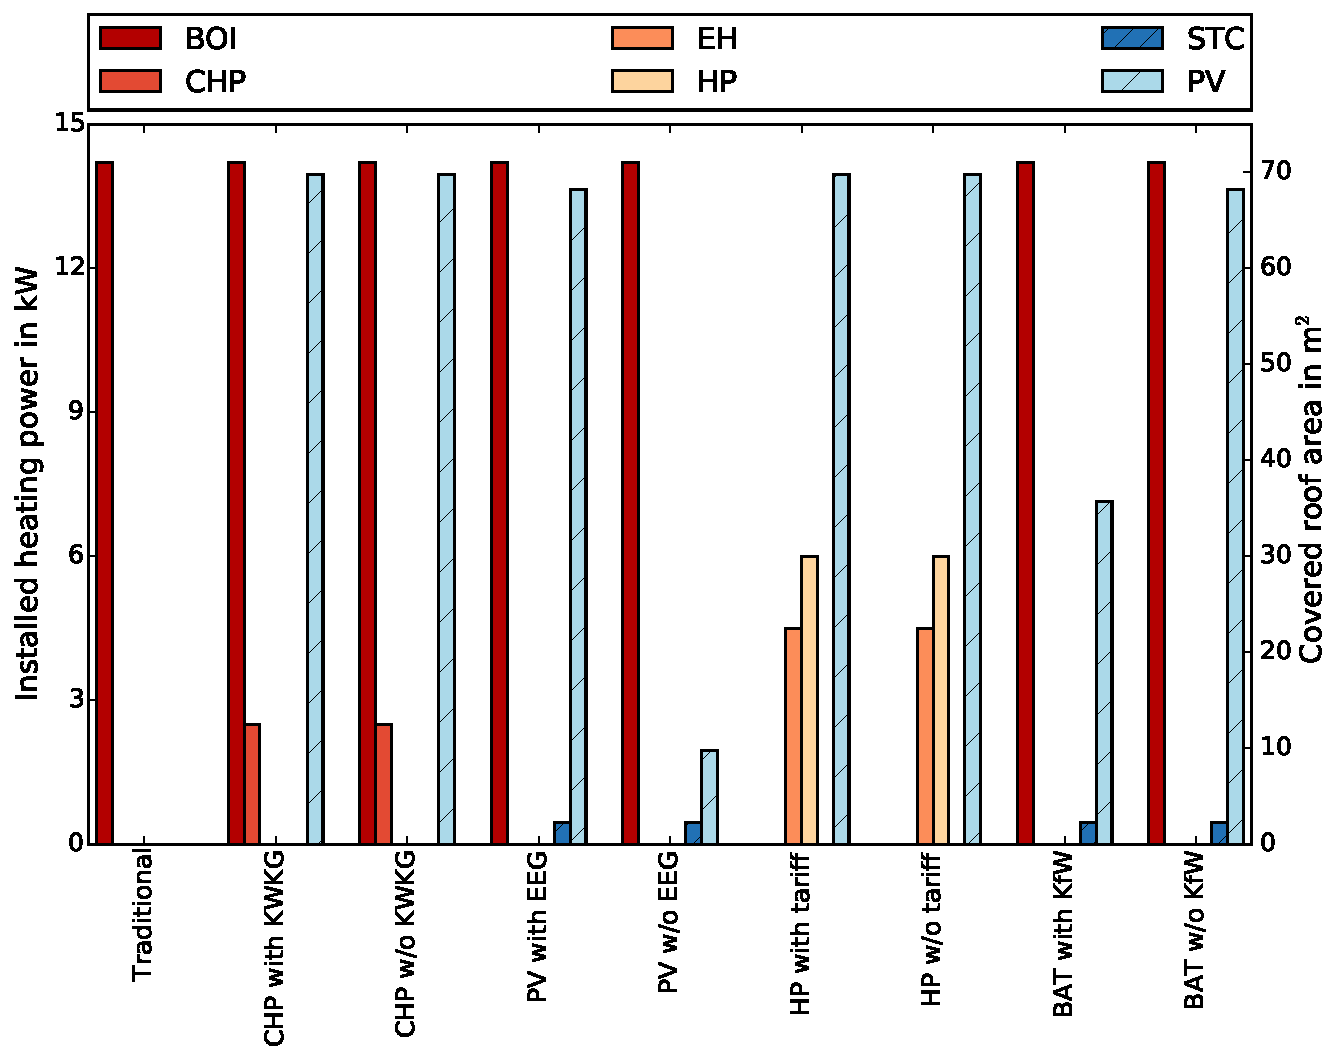
\includegraphics[width=\textwidth]{figures/plot_cap_gen_other.pdf}
		\caption{Rated powers (other) (double column figure)}
		\label{fig: heat generation other}
	\end{center}
\end{figure*}